\chapter{Teori, Sejarah, \& Instalasi Python}
\section{Teori}
Python adalah bahasa pemrograman interpretatif multiguna, python lebih menekankan pada keterbacaan kode agar lebih mudah untuk memahami sintaks.
\section{Sejarah Python}
Python diciptakan oleh Guido van Rossum pertama kali di centrum wiskunde \& informatica (CWI) di Belanda pada awal tahun 1990-an. bahasa yang terinpirasi dari bahasa pemograman ABC, hingga sampai saat ini Guido van Rossum menjadi penulis utama untuk phyton.
Tahun 1995 masih melanjutkan pembuatan phyton di Corporation for National Research Initiative (CNRI) di Virginia Amerika yang meriliskan beberapa bahasa phyton. Diantaranya :
\begin{enumerate}
	\item Python 1.0
	\\ Diliris pada januari tahun 1994
	\item Python 2.0
	\\ Diliris pada 16 Oktober tahun 2000
	\item Python 3.0 
	\\ Diliris pada 3 Desember tahun 2008
\end{enumerate}  
\subsubsection{Penggunaan Python di Perusahaan}
Salah satu bahasa yang banyak dipakai dalam sebuah perusahaan hingga saat ini yaitu bahasa pemograman python,  contoh penggunaan dalam perusahaan yaitu : 
\begin{enumerate}
\item Facebook
\\ Menggunakan framework python "Tornado" yang digunakan untuk menampilkan timeline
\item Instagram 
\\ Menggunakan framework python "Django" yang digunakan sebagai mesin pengelola sisi server dari aplikasi
\item Rasberry pi 
\\ Merupakan perangkat komputer mini yang digunakan sebagi mikrokontroler, bahasa yang digunakannya adalah python
\item NASA
\\ Badan antariksa Amerika ini menggunakan Python untuk bidang sainsnya.
\end{enumerate}
\subsubsection{Perbedaan Python 2 dan 3}
	Python 2 dipublikasikan pada akhir tahun 2000, dinilai lebih transparan dan inklusif untuk pengembangan software ketimbang versi sebelumnya. didukung dengan adanya PEP – Python Enhancement Proposal, dan dilengkapi dengan berbagai fitur programatikal seperti cycle-detecting garbage collector untuk mengotomasi manajemen memori. 
\\ Python 3 merupakan versi yang saat  ini dibuat masih aktif, versi ini banyak perubahan yang dirilis akhir tahun 2008. Fokus dari Python 3 itu sendiri adalah untuk melakukan perapian pada codebase dan menghapuskan duplikasi (redundancy). Python 3 mengalami hambatan pada pengadopsiannya, yang mengakibatkan tidak adanya backwards compatibility dengan Python 2.
\\	 
perbedaan yang mencolok terletak pada : 
\begin{enumerate}
\item Syntak
\item Pembagian pada integer
\end{enumerate}

\section{Instalasi}
\subsection{Instalasi Anaconda}
Berikut ini merupakan tutorial cara menginstalasi Anaconda, yang telah di download di www.anaconda.com setelah itu ikuti langkah-langkah dibawah ini.

	\begin{figure}
	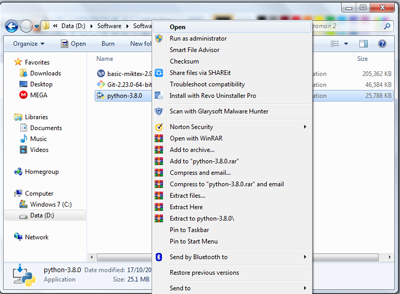
\includegraphics[scale=0.5]{section/1.png}
	\centering
	\caption{Tahap Instalasi 1}
	\end{figure}
	
	\begin{figure}
	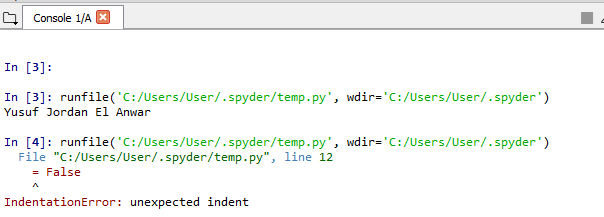
\includegraphics[scale=0.5]{section/2.png}
	\centering
	\caption{Tahapan Instalasi 2}
	\end{figure}

	\begin{figure}
	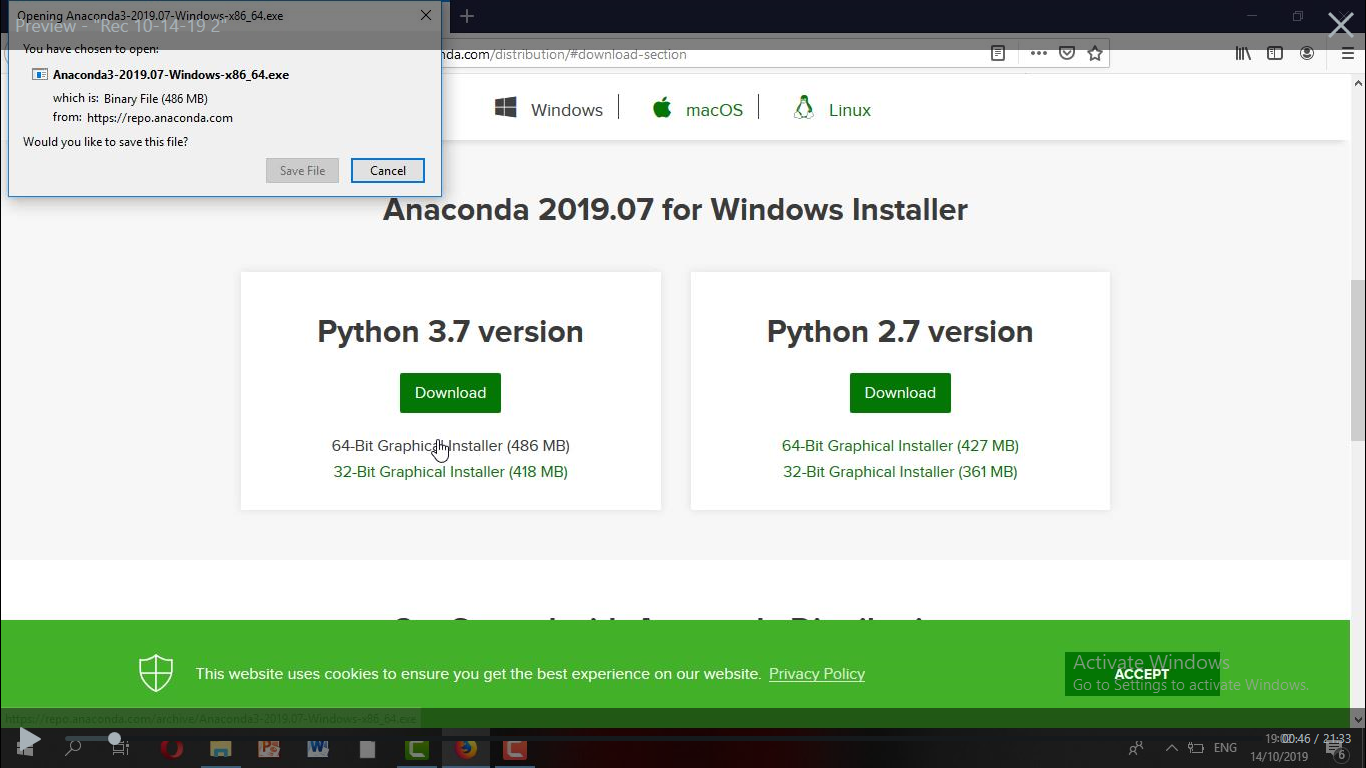
\includegraphics[scale=0.5]{section/3.png}
	\centering
	\caption{Tahapan Instalasi 3}
	\end{figure}

	\begin{figure}
	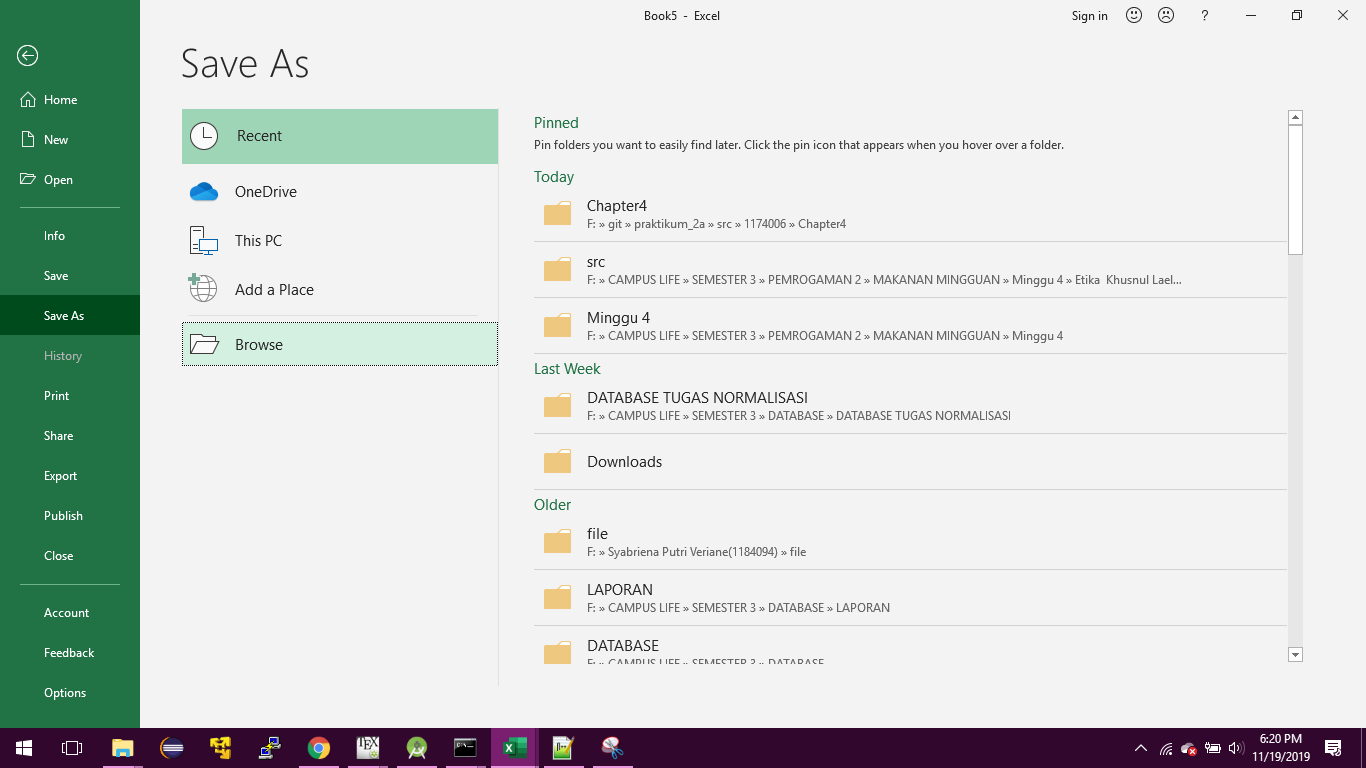
\includegraphics[scale=0.5]{section/4.png}
	\centering
	\caption{Tahapan Instalasi 4}
	\end{figure}

	\begin{figure}
	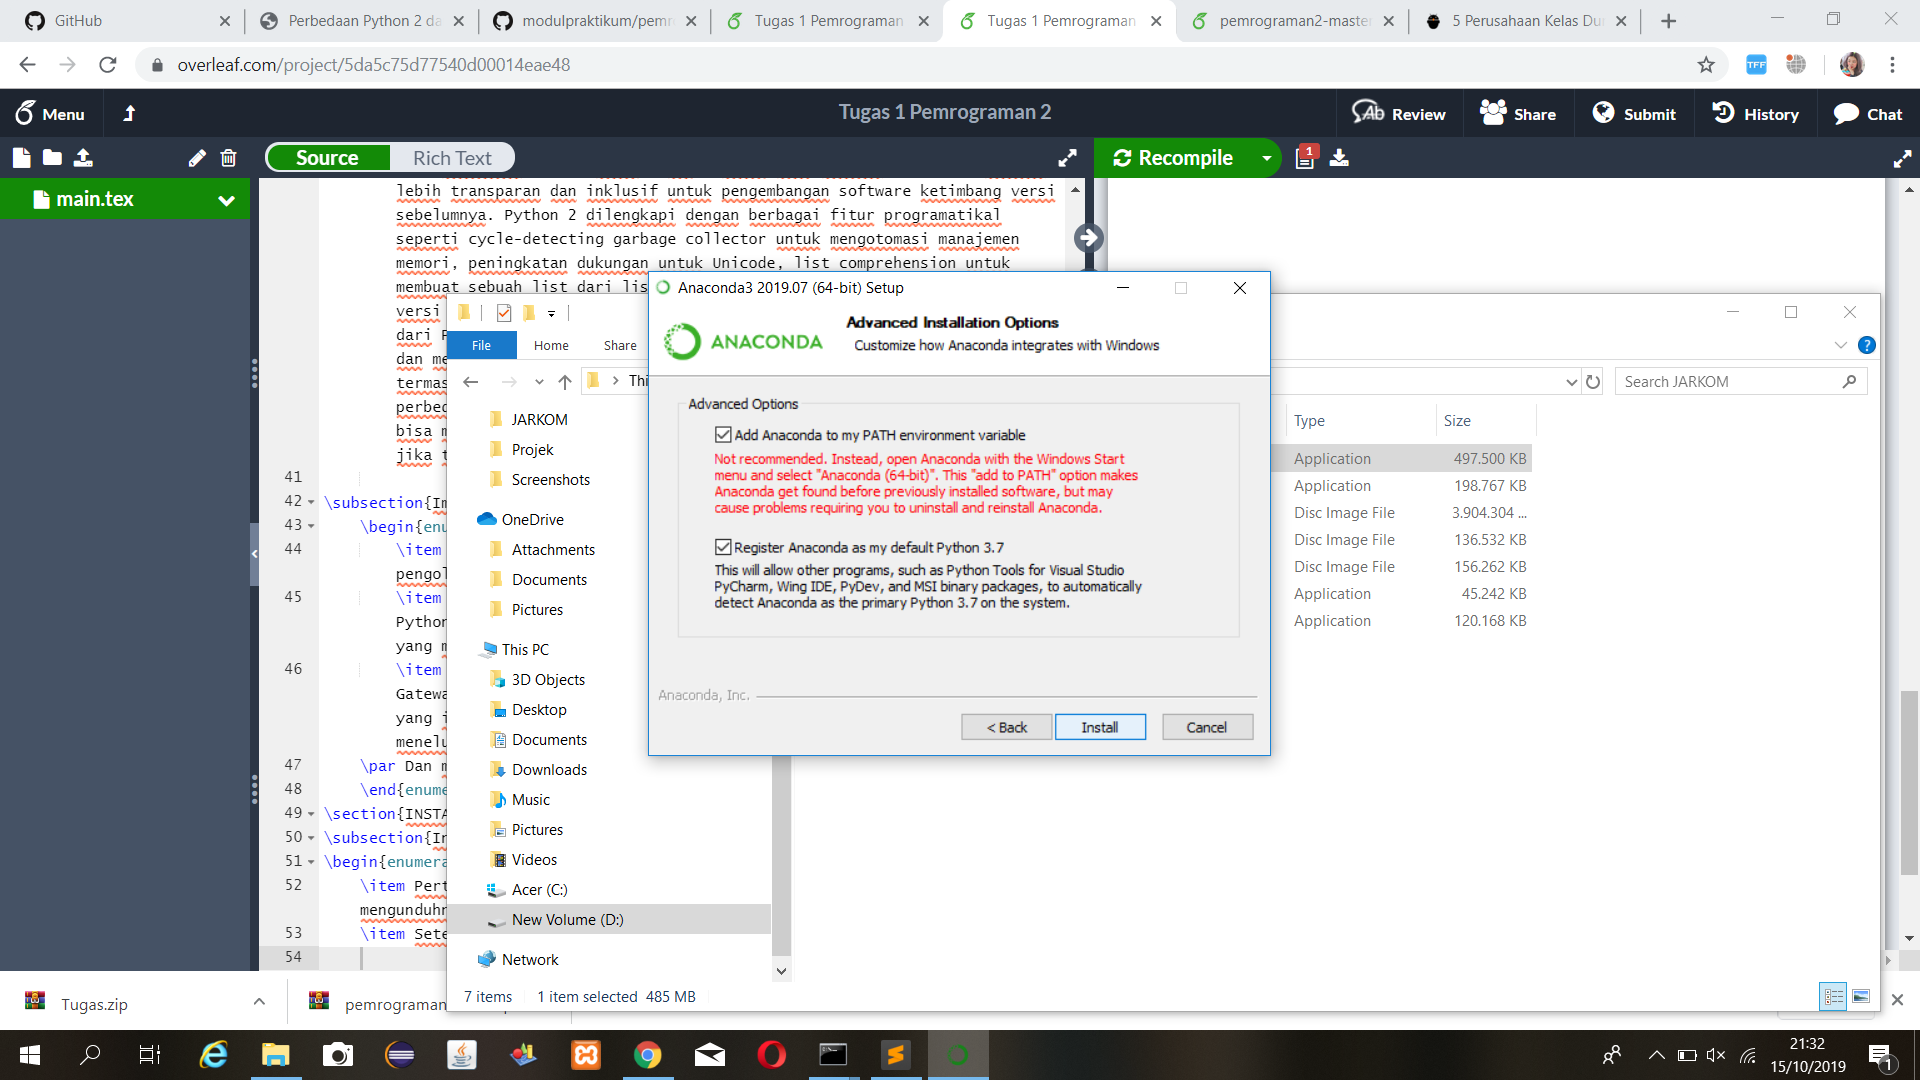
\includegraphics[scale=0.5]{section/5.png}
	\centering
	\caption{Tahapan Instalasi 5}
	\end{figure}

	\begin{figure}
	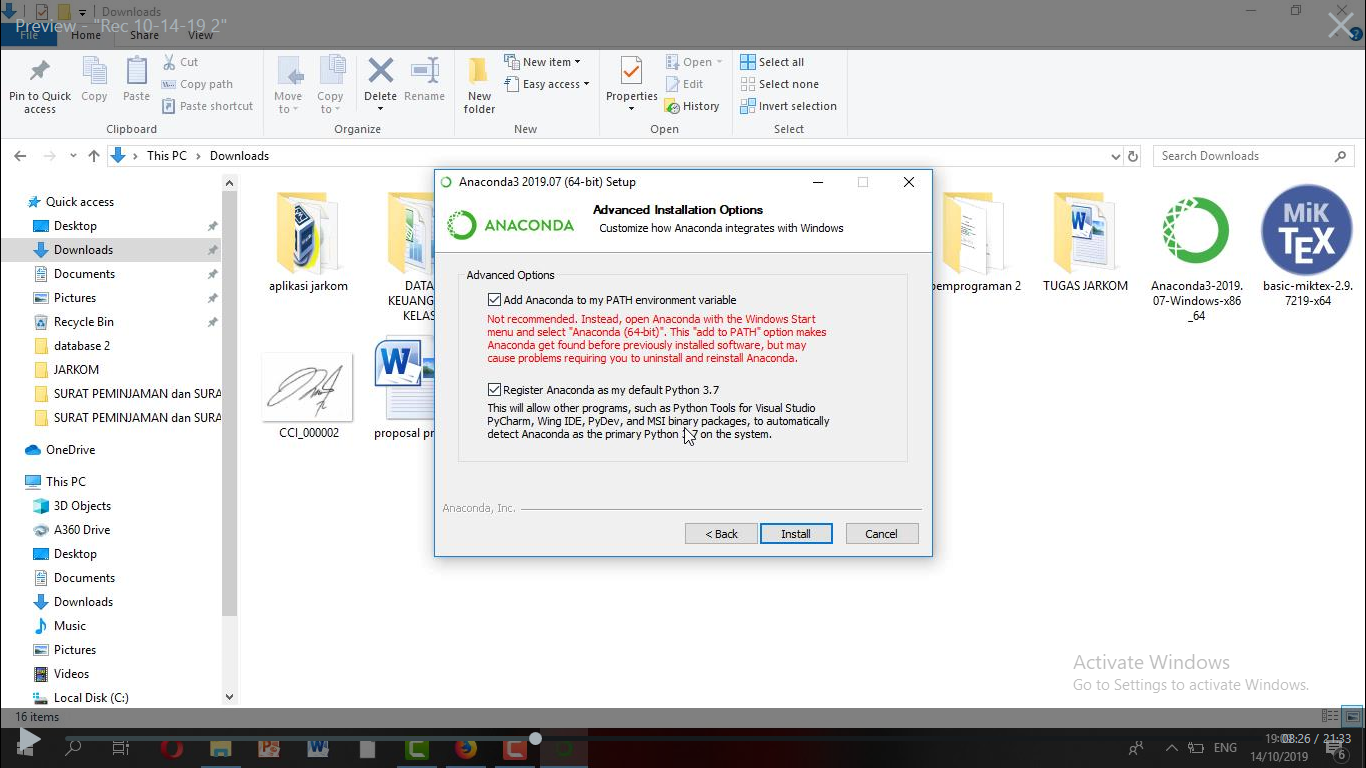
\includegraphics[scale=0.5]{section/6.png}
	\centering
	\caption{Tahapan Instalasi 6}
	\end{figure}

	\begin{figure}
	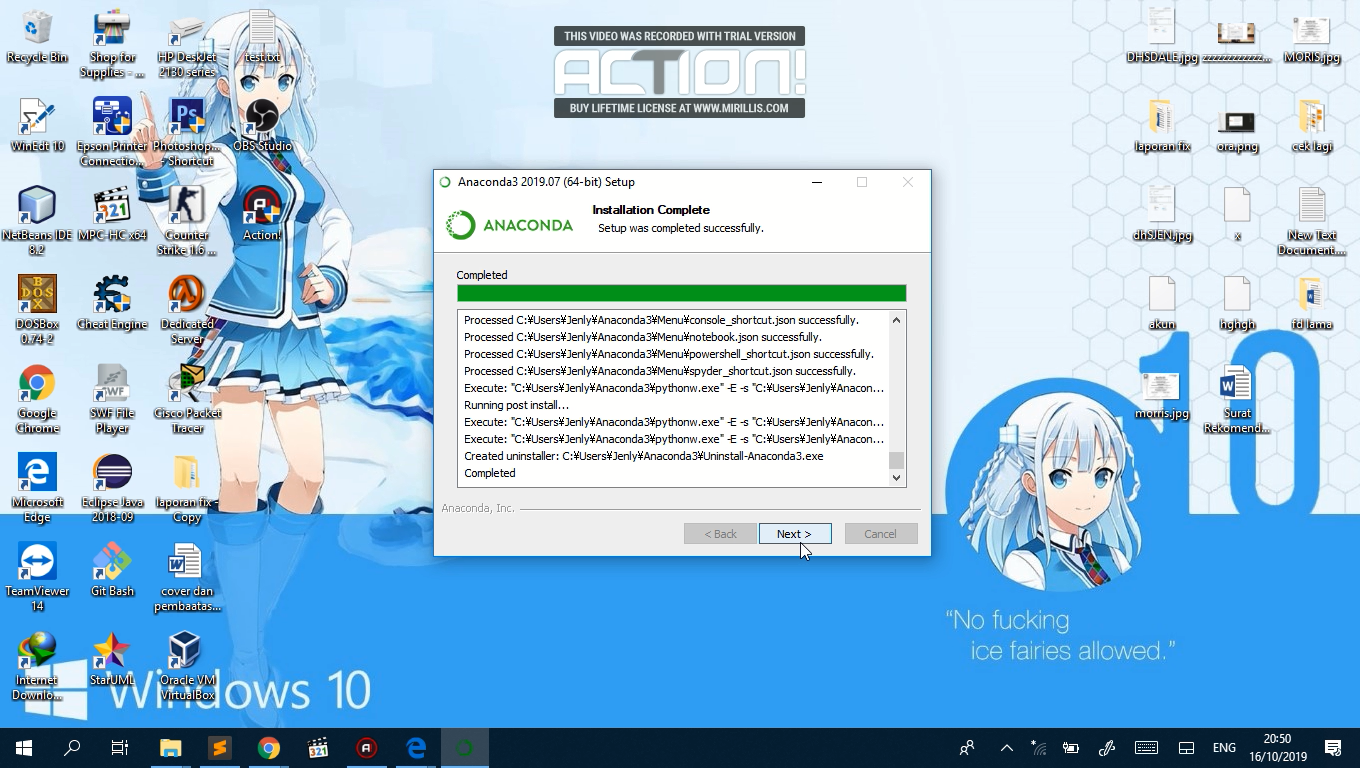
\includegraphics[scale=0.5]{section/7.png}
	\centering
	\caption{Tahapan Instalasi 7}
	\end{figure}

	\begin{figure}
	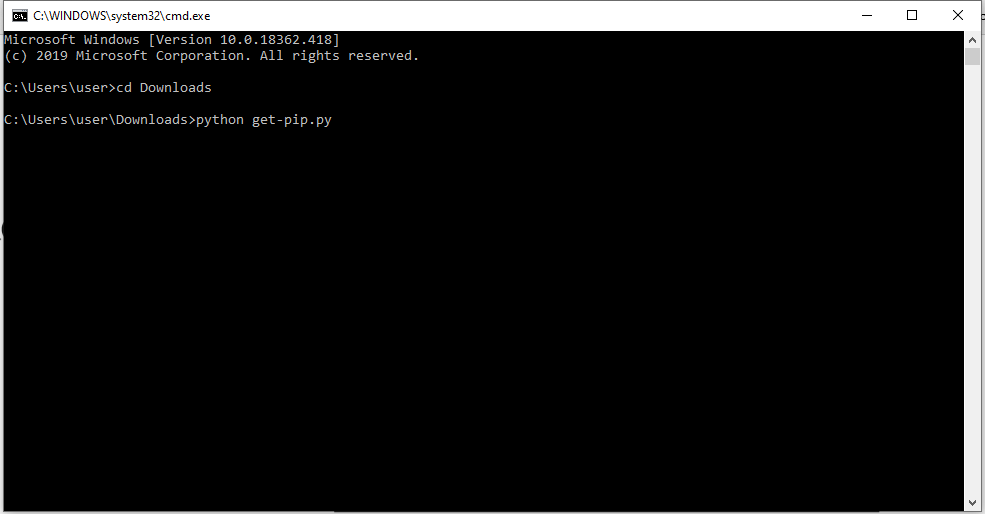
\includegraphics[scale=0.5]{section/8.png}
	\centering
	\caption{Tahapan Instalasi 8}
	\end{figure}

	\begin{figure}
	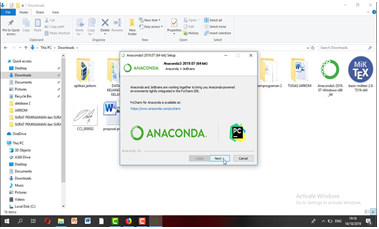
\includegraphics[scale=0.5]{section/9.png}
	\centering
	\caption{Tahapan Instalasi 9}
	\end{figure}

\subsection{Intalasi PIP}
Langkah-langkah mengisntall PIP

	\begin{figure}
	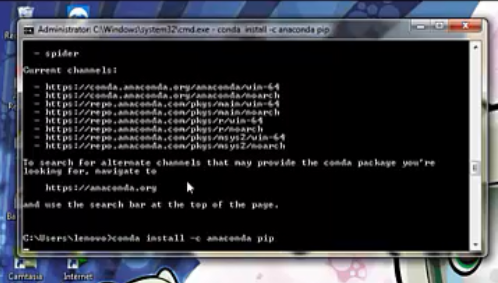
\includegraphics[scale=0.5]{section/pip1}
	\centering
	\caption{Ketik printah : conda install -c anaconda pip}
	\end{figure}
	
	\begin{figure}
	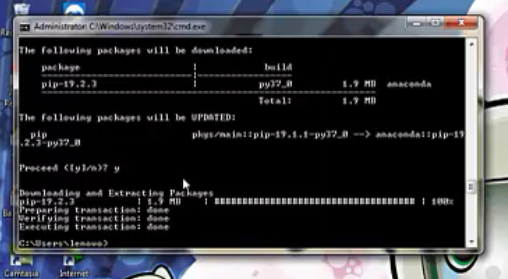
\includegraphics[scale=0.5]{section/pip2}
	\centering
	\caption{Tunggu hingga selesai}
	\end{figure}
	
\section{Setting Environment}
Langkah-langkah seperti ini : 

	\begin{figure}
	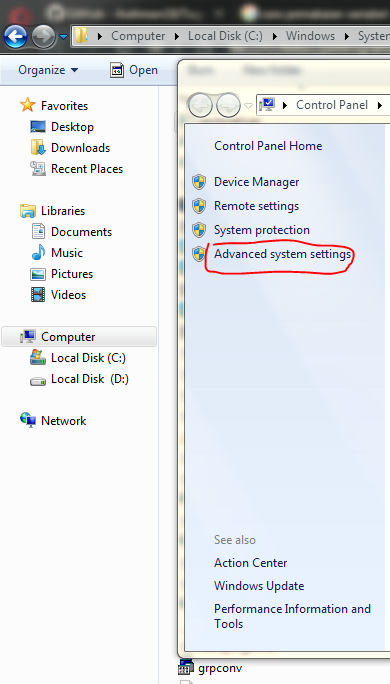
\includegraphics[scale=0.5]{section/envirotment1}
	\centering
	\caption{pilih advanced system setting}
	\end{figure}	
	
	\begin{figure}
	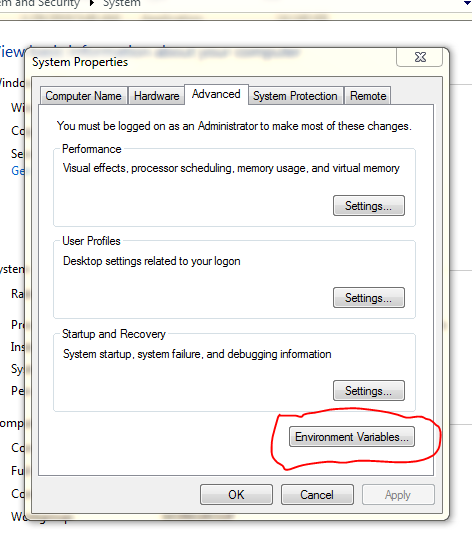
\includegraphics[scale=0.5]{section/envirotment2}
	\centering
	\caption{pilih envirotmet variabel}
	\end{figure}
	
	\begin{figure}
	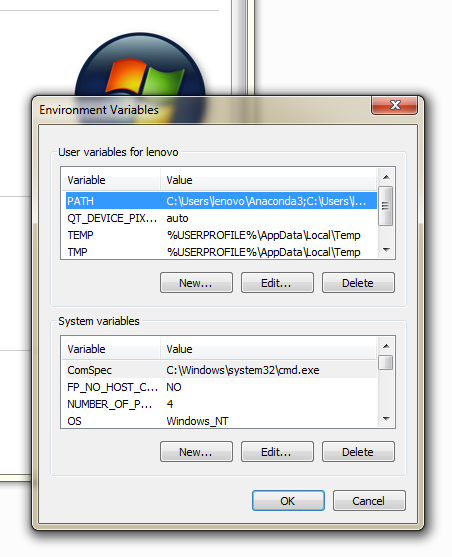
\includegraphics[scale=0.5]{section/envirotment3}
	\centering
	\caption{setting environment}
	\end{figure}
\section{Entrepreter atau CLI melalui terminal atau cmd windows}
pada tahap ini, dibutuhkanya cmd sebagai bahan pembelajaran dari mulai cek status python yang sudah terbaru, hingga proses pengupdatetan seperti contoh dibawah ini:

	\begin{figure}
	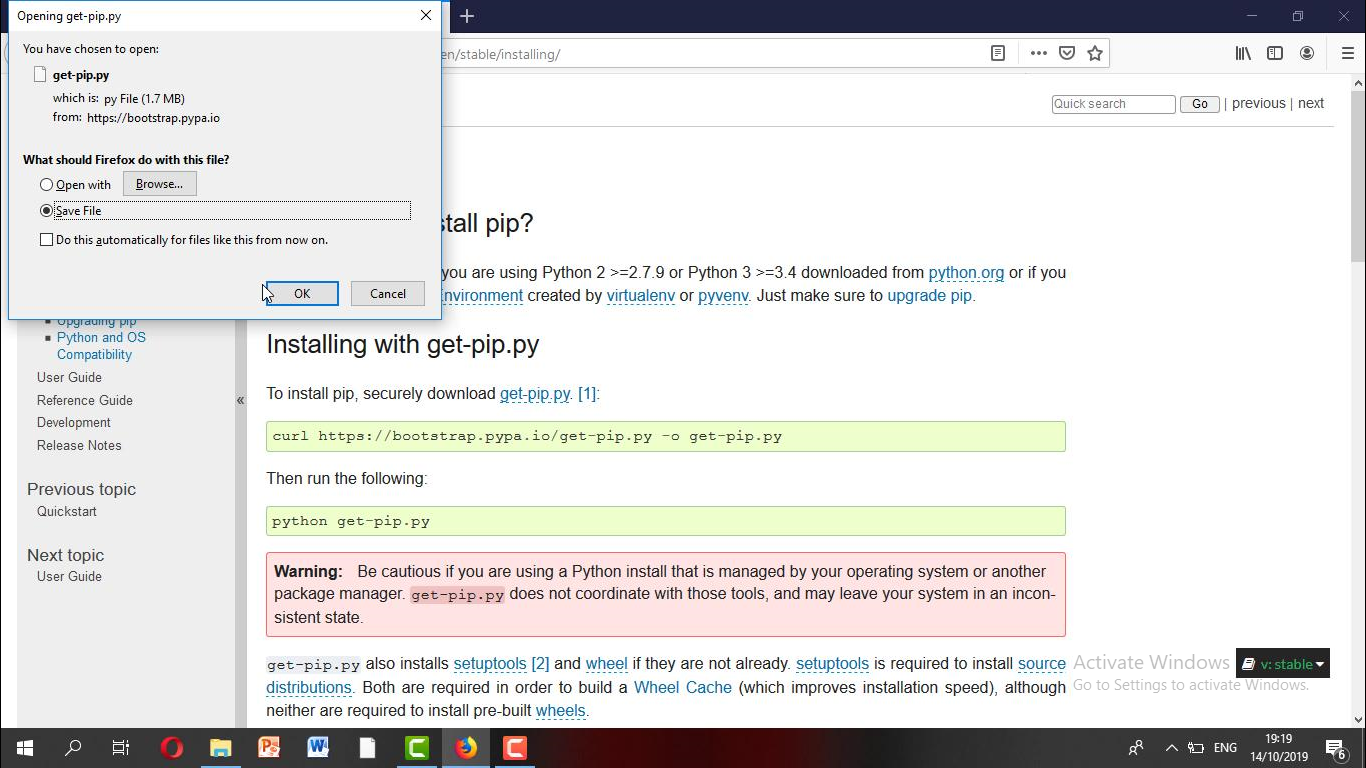
\includegraphics[scale=0.5]{section/13.png}
	\centering
	\caption{Tahapan Cek python}
	\end{figure}

	\begin{figure}
	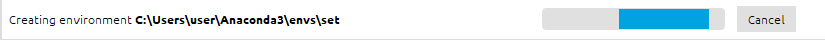
\includegraphics[scale=0.5]{section/14.png}
	\centering
	\caption{Tahapan pengudatetan}
	\end{figure}

\section{Mengupdate Spyder}
Pada langkah ini, dibutuhkan sebuah command Prompt dengan megetikkan
\\ conda install -c anaconda spyder

	\begin{figure}
	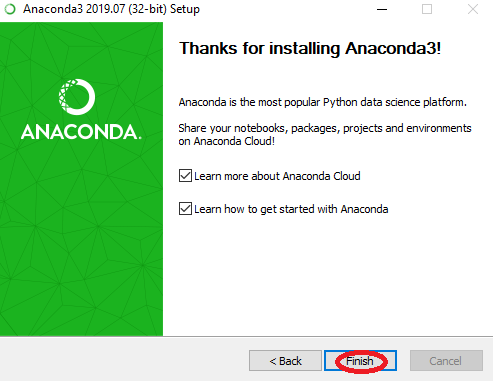
\includegraphics[scale=0.5]{section/10.png}
	\centering
	\caption{Tahapan update spyder}
	\end{figure}

\section{Menjalankan Hello World}
Pada langkah ini harus di siapkan spyder yang digunakan sebagai text editor yang membantu menerjemahkan bahasa pemograman python, diantaranya sebagai berikut :

	\begin{figure}
	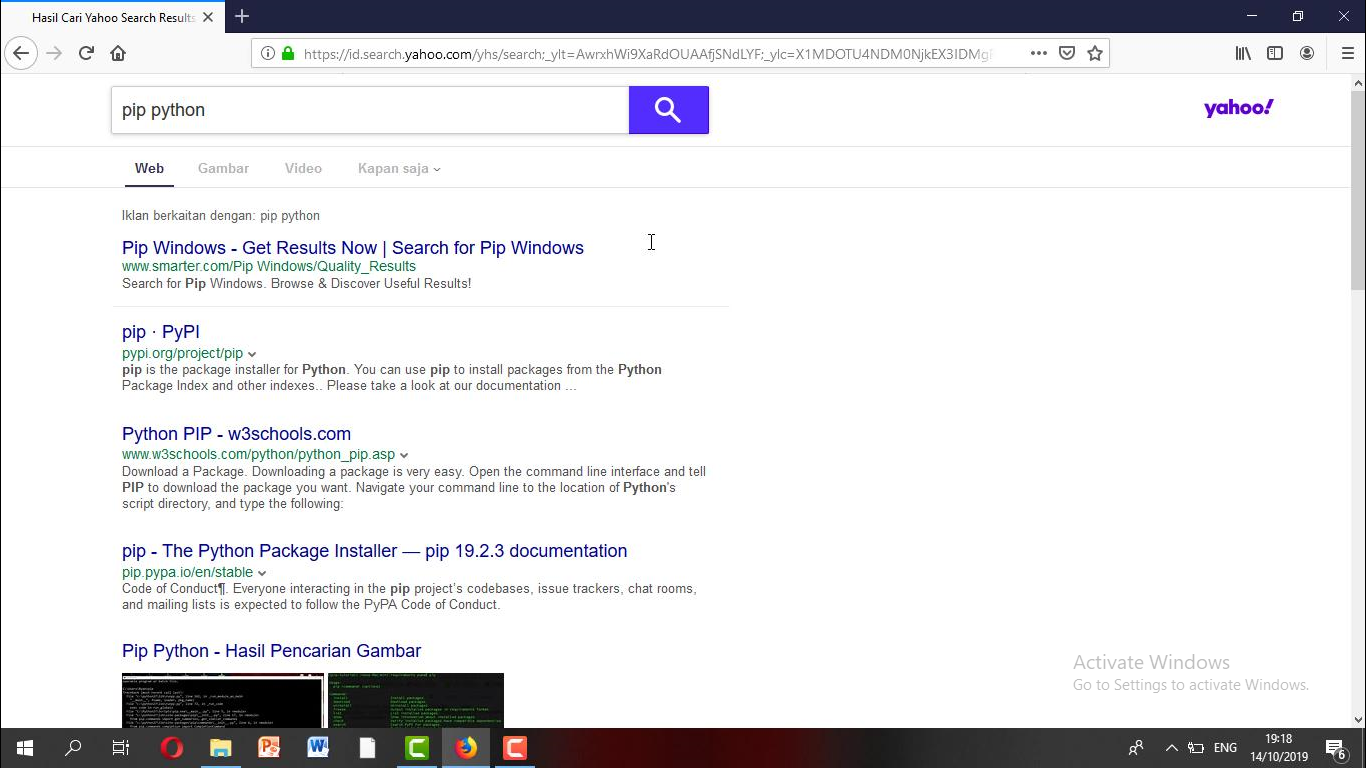
\includegraphics[scale=0.5]{section/11.png}
	\centering
	\caption{Syntak hello world}
	\end{figure}

	\begin{figure}
	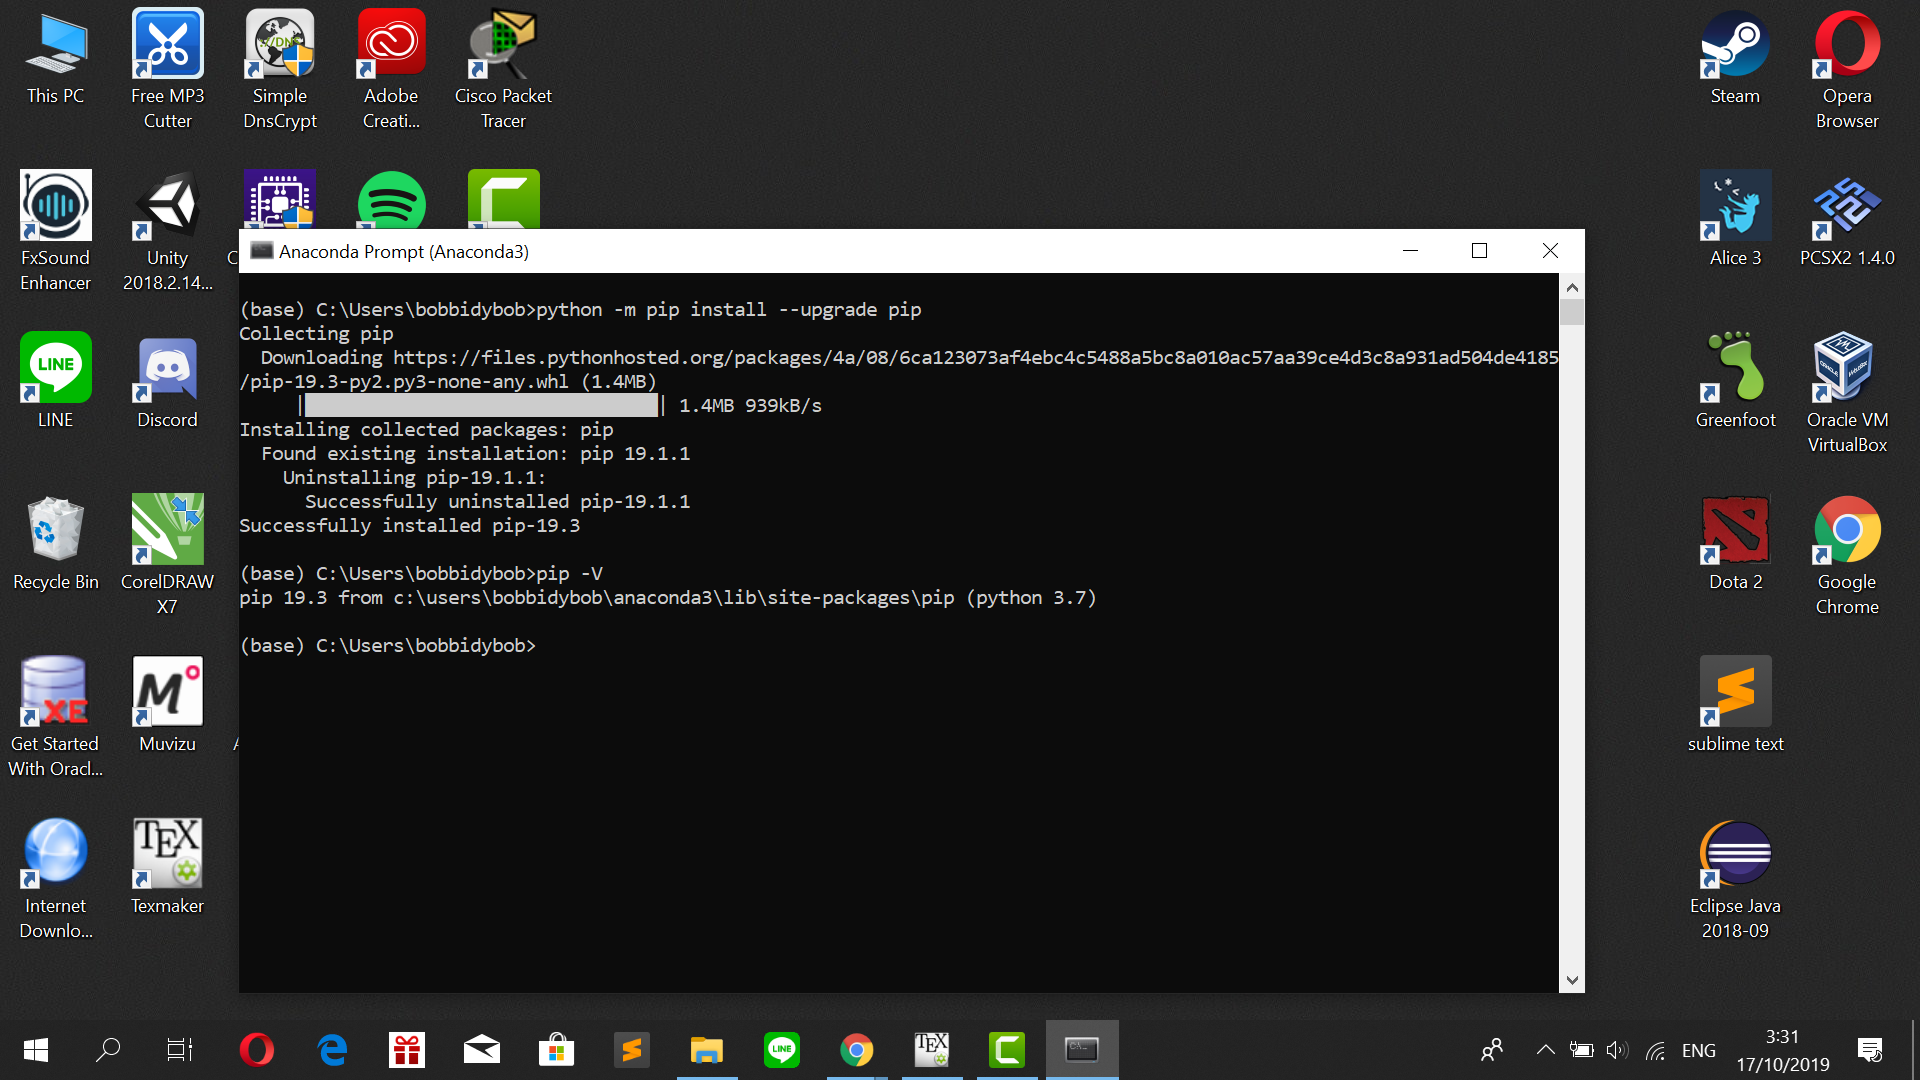
\includegraphics[scale=0.5]{section/12.png}
	\centering
	\caption{menampilkan hello world}
	\end{figure}


\section{Menjalankan Script Otomatis Login Aplikasi Akademik}
Pada langkah pertama instal selenium terlebih dahulu seperti contoh ini :

	\begin{figure}
	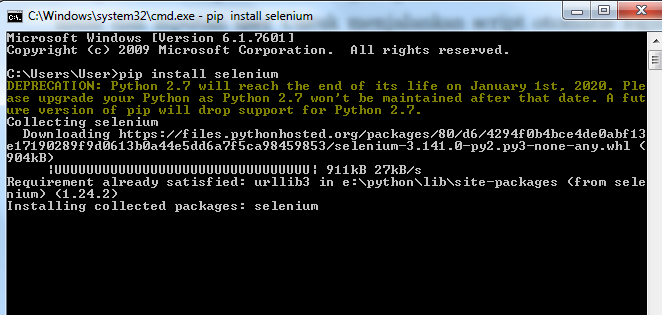
\includegraphics[scale=0.5]{section/selenium.png}
	\centering
	\caption{Install selenium}
	\end{figure}

	\begin{figure}
	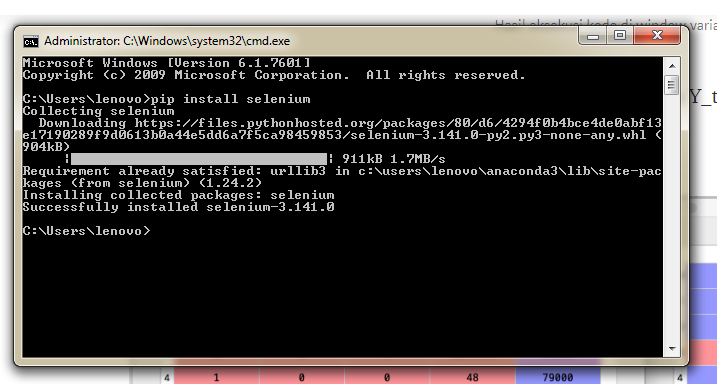
\includegraphics[scale=0.5]{section/proses_selenium}
	\centering
	\caption{Tahap instalasi selenium}
	\end{figure}
	
	\begin{figure}
	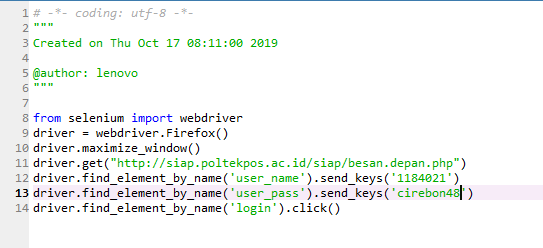
\includegraphics[scale=0.5]{section/login_otomatis}
	\centering
	\caption{Syntak pada spyder untuk otomatis login}
	\end{figure}
	
	\begin{figure}
	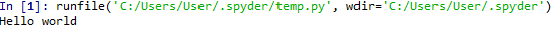
\includegraphics[scale=0.3]{section/hasil.png}
	\centering
	\caption{hasil}
	\end{figure}

\section{Variable Explorer}
Variabel explorer digunakan sebagai bawaan untuk mengedit daftar, string, kamus, array NumPy, Pandas DataFrames, dan banyak lagi, dan dapat juga histogram, plot, atau bahkan menampilkan beberapa di antaranya sebagai gambar RGB. Bisa dicek dengan mengklik variabel explorer pada spyder.

	\begin{figure}
	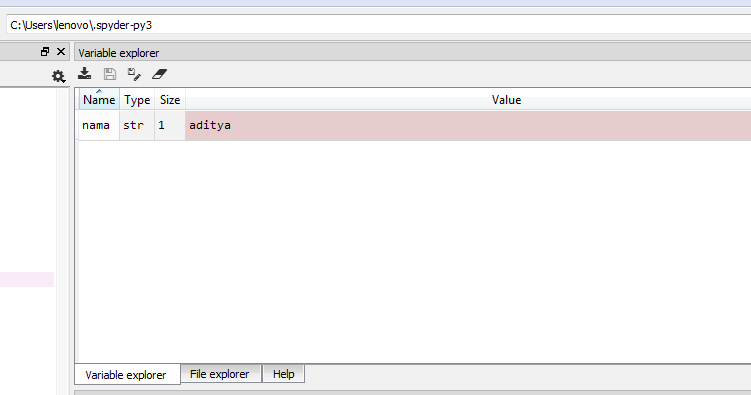
\includegraphics[scale=0.3]{section/variabel_explorer.png}
	\centering
	\caption{cek variabel explorer}
	\end{figure}
	
\section{Identasi}
Indentasi adalah bagian paragraf yang menjorok ke dalam pada baris-baris
paragraf, penulisan kode python tidak memakai curly brackets ”{}” sehingga
cara membedakan blok program digunakan identasi.
jenis error identasi yaitu IndentationError: expected an indented block.
artinya ini berarti fungsi if memerlukan indentasi untuk membedakan blok
kode.

	\begin{figure}
	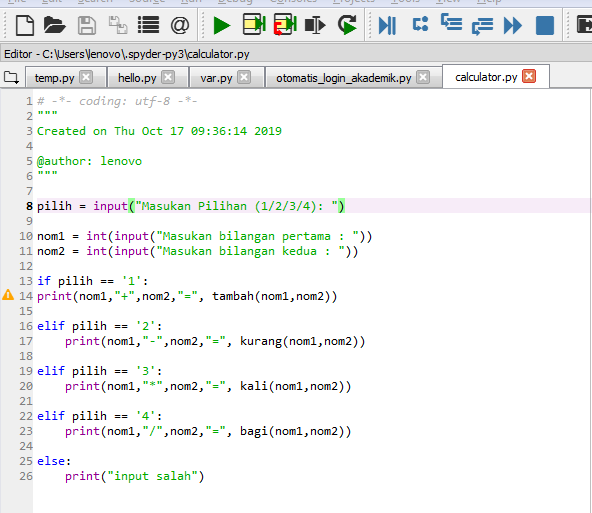
\includegraphics[scale=0.5]{section/salah.png}
	\centering
	\caption{syntak eror identasi}
	\end{figure}
	
	\begin{figure}
	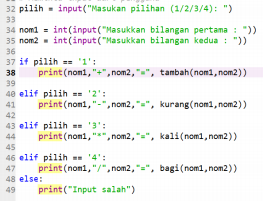
\includegraphics[scale=1.5]{section/benar.png}
	\centering
	\caption{cek variabel explorer}
	\end{figure}